\documentclass[12pt,a4paper]{article}
\usepackage[UTF8, heading=true]{ctex}
\usepackage{geometry}
\usepackage{multirow}
\usepackage{booktabs}
\usepackage{graphicx}
\usepackage{float}
\usepackage{listings}
\usepackage{tikz}
\usetikzlibrary{shapes.geometric, arrows, positioning, calc}
\lstset{
    basicstyle=\small\ttfamily,
    breaklines=true,
    columns=flexible,
    keepspaces=true
}
% 页边距设置
\geometry{left=2.5cm,right=2.5cm,top=2.5cm,bottom=2.5cm}
% 字体与行距设置
\ctexset{
    section = { format=\bfseries\large },
    subsection = { format=\bfseries\normalsize }
}
\linespread{1.5}
\fontsize{10.5pt}{12pt}\selectfont

\begin{document}
% 标题
\begin{center}
    \textbf{\small 智能垃圾分类处理系统仿真程序设计}
\end{center}

% 基本信息
\noindent
\textbf{成  绩}\hspace{4cm} \textbf{指导教师}：罗志祥 \\
\textbf{专业班级}：光电信息科学与工程202409 \hspace{1cm} \textbf{姓  名}：陈恪瑾 \hspace{1cm} \textbf{学  号}：U202413925 \\
\textbf{联系电话}：18571851291

\section{任务要求}
\subsection{实验目的}
\begin{itemize}
    \item 掌握 AT89S52 定时器、中断等外设的基本使用方法；
    \item 理解智能垃圾桶控制系统的设计逻辑与状态转换过程。
\end{itemize}

\subsection{实验内容}
在 Keil 环境中设计一个基于 AT89S52 单片机的智能垃圾分类处理系统。用户通过 P2 口输入、P1 口输出（上电复位初始状态为全 1），模拟小区垃圾回收终端运行状态。系统需满足以下功能：
\begin{itemize}
    \item 在实验一的基础上修改并扩展设计代码；
    \item 居民通过按键选择垃圾类型（P2.7、P2.6、P2.5、P2.4 低电平有效，分别对应塑料纸张、玻璃金属、厨余垃圾、危害垃圾）；
    \item P1.0$\sim$P1.3 控制四个垃圾桶盖，高电平为关闭状态，低电平为打开状态；
    \item 每次开盖持续 8s 后自动关闭，采用定时器中断程序实现延时，计时精度达到 1ms 以内；
    \item 开盖 8s 期间，P0 口 8 位按剩余时间依次由 1 变至 0，作为开盖进度条显示。
\end{itemize}
请编写程序，实现用户键入后对应垃圾桶盖的打开与关闭控制。

\subsection{提高部分（申优选做）}
\begin{itemize}
    \item 系统初始化后随机生成 4 个 $0\sim9$ 的整数，置于寄存器 R0$\sim$R3 表示四个垃圾桶剩余容量；每次投递后容量相应减少。投放超出剩余容量后，对应标志位发生变化（自行定义），用于提醒物业清理；再次按键时该桶盖不再打开以避免溢出。
    \item 自行定义清理键，按下后所有垃圾桶容量恢复为 9，溢出标志位恢复初值。
    \item 在垃圾桶盖打开的 8s 内，用户可通过按键触发中断（自行设置），停止计时并提前关闭桶盖。
    \item 其他个性化设计。
\end{itemize}

\section{设计思路}
本系统基于 AT89S52 单片机，采用“主循环轮询 + 定时器中断 + 外部中断”的协同控制方式，围绕垃圾分类投放需求划分功能模块，整体设计逻辑如下：
\begin{enumerate}
    \item \textbf{系统初始化模块}：上电后将 P1 置为 0xFF（桶盖全关）、P0 清零、P2 置 0xFF；清空满载标志字节 FULL\_FLAGS 并刷新满载指示灯。随后配置 TMOD=11H（T0/T1 均为模式1），开启 ET0、EX0 和总中断 EA：其中 T0 用于 1ms 节拍计时，INT0（P3.2）用于“提前关盖”外部中断。T1 保持运行，为随机容量生成提供硬件扰动。
    \item \textbf{主循环按键调度模块}：主循环首先检测清理键 P2.3，按下后将 R0$\sim$R3 容量恢复为 9，并清除满载标志；若未清理，则轮询 P2.7$\sim$P2.4 四类投放键，检测到低电平后跳转到对应 TRY\_BINx 分支执行投放处理。
    \item \textbf{投放与容量管理模块}：在 TRY\_BINx 中先判断对应满载位，满载则拒绝开盖；未满时检查容量寄存器，容量为 0 则立即置满载标志；否则容量减 1，若减到 0 同步置满载并刷新指示灯。通过上述逻辑实现“容量递减、满载封桶、防溢出”的闭环控制。
    \item \textbf{8 秒开盖窗口与进度显示模块}：OPEN\_BIN\_8S 子程序接收桶盖位掩码，拉低 P1 对应位开盖，并初始化 SEC\_LEFT=8、MS\_CNT=03E8H 与 PROGRESS=FFH。开盖期间由 Timer0 每 1ms 中断递减毫秒计数；每累计 1 秒，P0 进度字节右移一位（FF$\rightarrow$7F$\rightarrow$3F$\rightarrow\cdots\rightarrow$00），SEC\_LEFT 递减；当 SEC\_LEFT 减至 0 时自动调用 FORCE\_CLOSE 关盖。
    \item \textbf{提前关盖中断模块}：用户在 8 秒窗口内按下提前关盖键（INT0/P3.2 下降沿触发）进入 EXT0\_ISR。中断服务程序在 OPENING=1 时立即调用 FORCE\_CLOSE，停止 T0 计时并关闭当前桶盖，从而实现“投放完成即中断关盖”的实时响应。
    \item \textbf{随机数与满载指示模块}：随机子程序读取 TL1/TH1，并经异或、移位与模10处理生成 0$\sim$9 初值写入 R0$\sim$R3。满载指示由 UPDATE\_FULL\_LED 完成：考虑 P3.2 已被 INT0 占用，程序将四个满载位映射到 P3.0、P3.1、P3.4、P3.5 输出。
\end{enumerate}

\section{资源分配}
\subsection{I/O口硬件资源分配}
\begin{table}[H]
    \centering
    \small
    \begin{tabular}{|c|c|c|c|}
        \hline
        I/O引脚 & 方向 & 功能定义 & 有效电平 \\
        \hline
        P1.0 & 输出 & 塑料纸张垃圾桶盖控制 & 低电平打开，高电平关闭 \\
        \hline
        P1.1 & 输出 & 玻璃金属垃圾桶盖控制 & 低电平打开，高电平关闭 \\
        \hline
        P1.2 & 输出 & 厨余垃圾垃圾桶盖控制 & 低电平打开，高电平关闭 \\
        \hline
        P1.3 & 输出 & 危害垃圾桶盖控制 & 低电平打开，高电平关闭 \\
        \hline
        P2.3 & 输入 & 一键清理复位按键 & 低电平有效 \\
        \hline
        P2.4 & 输入 & 危害垃圾投放按键 & 低电平有效 \\
        \hline
        P2.5 & 输入 & 厨余垃圾投放按键 & 低电平有效 \\
        \hline
        P2.6 & 输入 & 玻璃金属投放按键 & 低电平有效 \\
        \hline
        P2.7 & 输入 & 塑料纸张投放按键 & 低电平有效 \\
        \hline
        P0.0$\sim$P0.7 & 输出 & 8秒开盖进度条显示 & 高位到低位逐步由1变0 \\
        \hline
        P3.0 & 输出 & 塑料纸张满载指示信号 & 高电平点亮 \\
        \hline
        P3.1 & 输出 & 玻璃金属满载指示信号 & 高电平点亮 \\
        \hline
        P3.2/INT0 & 输入 & 提前关盖外部中断按键 & 下降沿触发 \\
        \hline
        P3.4 & 输出 & 厨余垃圾满载指示信号 & 高电平点亮 \\
        \hline
        P3.5 & 输出 & 危害垃圾满载指示信号 & 高电平点亮 \\
        \hline
    \end{tabular}
\end{table}

\subsection{寄存器资源分配}
\begin{table}[H]
    \centering
    \small
    \begin{tabular}{|c|c|}
        \hline
        寄存器 & 功能定义 \\
        \hline
        R0 & 塑料纸张垃圾桶剩余容量（0$\sim$9） \\
        \hline
        R1 & 玻璃金属垃圾桶剩余容量（0$\sim$9） \\
        \hline
        R2 & 厨余垃圾桶剩余容量（0$\sim$9） \\
        \hline
        R3 & 危害垃圾桶剩余容量（0$\sim$9） \\
        \hline
        A & 指令运算、端口读写、掩码处理与中间数据暂存 \\
        \hline
        TH0, TL0 & Timer0 1ms节拍重装与计时（FC18H重装） \\
        \hline
        TH1, TL1 & Timer1自由运行计数，作为随机数扰动源 \\
        \hline
    \end{tabular}
\end{table}

\subsection{片内RAM资源分配}
\begin{table}[H]
    \centering
    \small
    \begin{tabular}{|c|c|}
        \hline
        存储单元 & 功能定义 \\
        \hline
        20H（FULL\_FLAGS） & 四个垃圾桶满载标志字节（bit0$\sim$bit3） \\
        \hline
        21H（TMP\_DATA） & LED刷新与位映射过程的临时缓存 \\
        \hline
        22H（MS\_CNT\_L） & 1秒计数低字节（03E8H低位） \\
        \hline
        23H（MS\_CNT\_H） & 1秒计数高字节（03E8H高位） \\
        \hline
        24H（SEC\_LEFT） & 开盖剩余秒数（初始化为8） \\
        \hline
        25H（PROGRESS） & P0进度条显示字节（FFH右移至00H） \\
        \hline
        26H（ACTIVE\_MASK） & 当前开盖桶的位掩码（01/02/04/08） \\
        \hline
        27H（STATE.0=OPENING） & 开盖状态位（1=正在开盖计时，0=关闭） \\
        \hline
    \end{tabular}
\end{table}

\section{流程图}
\subsection{主程序流程图}
\begin{figure}[H]
    \centering
    \small
    \resizebox{0.96\textwidth}{!}{%
    \begin{tikzpicture}[node distance=0.92cm and 2.2cm]
        \tikzstyle{startstop} = [rectangle, rounded corners, minimum width=2.5cm, minimum height=0.7cm,text centered, align=center, draw=black, fill=red!10]
        \tikzstyle{process} = [rectangle, minimum width=3.35cm, minimum height=0.7cm, text centered, align=center, draw=black, fill=blue!10]
        \tikzstyle{decision} = [diamond, aspect=2.1, minimum width=3.35cm, minimum height=0.8cm, text centered, align=center, draw=black, fill=green!10]
        \tikzstyle{arrow} = [thick,->,>=stealth]
        \tikzstyle{flowlabel} = [fill=white, inner sep=1pt]

        \node (start) [startstop] {开始};
        \node (init) [process, below=of start] {初始化端口/定时器/中断\\生成随机容量};
        \node (scan) [process, below=of init] {主循环扫描按键};
        \node (clearq) [decision, below=of scan] {P2.3清理键按下?};
        \node (clear) [process, left=2.9cm of clearq] {R0$\sim$R3$\leftarrow$9\\清满载标志并更新LED};
        \node (keyq) [decision, below=of clearq] {P2.7$\sim$P2.4有键按下?};
        \node (try) [process, below=of keyq] {进入TRY\_BINx分支};
        \node (fullq) [decision, below=of try] {对应满载位=1?};
        \node (capq) [decision, below=of fullq] {当前容量=0?};
        \node (dec) [process, below=of capq] {容量减1};
        \node (zeroq) [decision, below=of dec] {减1后为0?};
        \node (markdeny) [process, right=2.9cm of capq] {置满载位更新LED\\拒绝开盖};
        \node (markopen) [process, right=2.9cm of zeroq] {置满载位并更新LED};
        \node (open) [process, below=of zeroq] {OPEN\_BIN\_8S\\开盖并启动8s窗口};
        \node (wait) [decision, below=of open] {OPENING=1?};
        \node (rel) [process, left=2.9cm of wait] {按键释放等待};

        \coordinate (returnbus) at ($(clear.west)+(-0.75cm,0)$);
        \coordinate (fullbus) at ($(clear.west)+(-1.45cm,0)$);
        \coordinate (denybus) at ($(markdeny.east)+(0.75cm,0)$);
        \coordinate (denybottom) at ($(rel.south)+(0,-1.25cm)$);

        \draw [arrow] (start) -- (init);
        \draw [arrow] (init) -- (scan);
        \draw [arrow] (scan) -- (clearq);
        \draw [arrow] (clearq.west) -- node[flowlabel, above] {是} (clear.east);
        \draw [arrow] (clear.west) -- (returnbus |- clear.west) -- (returnbus |- scan.west) -- (scan.west);
        \draw [arrow] (clearq) -- node[flowlabel, right] {否} (keyq);
        \draw [arrow] (keyq.west) -- node[flowlabel, above, pos=0.25] {否} (returnbus |- keyq.west) -- (returnbus |- scan.west) -- (scan.west);
        \draw [arrow] (keyq) -- node[flowlabel, right] {是} (try);
        \draw [arrow] (try) -- (fullq);
        \draw [arrow] (fullq.west) -- node[flowlabel, above, pos=0.25] {是} (fullbus |- fullq.west) -- (fullbus |- rel.west) -- (rel.west);
        \draw [arrow] (fullq) -- node[flowlabel, right] {否} (capq);
        \draw [arrow] (capq.east) -- node[flowlabel, above] {是} (markdeny.west);
        \draw [arrow] (markdeny.east) -- (denybus |- markdeny.east) -- (denybus |- denybottom) -- (rel.south |- denybottom) -- (rel.south);
        \draw [arrow] (capq) -- node[flowlabel, right] {否} (dec);
        \draw [arrow] (dec) -- (zeroq);
        \draw [arrow] (zeroq.east) -- node[flowlabel, above] {是} (markopen.west);
        \draw [arrow] (markopen.south) |- (open.east);
        \draw [arrow] (zeroq) -- node[flowlabel, right] {否} (open);
        \draw [arrow] (open) -- (wait);
        \draw [arrow] (wait.south) -- ++(0,-0.55) -| node[flowlabel, pos=0.25, right] {是} (wait.east);
        \draw [arrow] (wait.west) -- node[flowlabel, above] {否} (rel.east);
        \draw [arrow] (rel.west) -- (returnbus |- rel.west) -- (returnbus |- scan.west) -- (scan.west);
    \end{tikzpicture}
    }
    \caption{主程序流程图}
\end{figure}

\subsection{Timer0中断服务流程图}
\begin{figure}[H]
    \centering
    \small
    \begin{tikzpicture}[node distance=1.25cm]
        \tikzstyle{startstop} = [rectangle, rounded corners, minimum width=3.2cm, minimum height=0.8cm,text centered, align=center, draw=black, fill=red!10]
        \tikzstyle{process} = [rectangle, minimum width=4.2cm, minimum height=0.8cm, text centered, align=center, draw=black, fill=blue!10]
        \tikzstyle{decision} = [diamond, aspect=2.3, minimum width=4.0cm, minimum height=0.9cm, text centered, align=center, draw=black, fill=green!10]
        \tikzstyle{arrow} = [thick,->,>=stealth]

        \node (in) [startstop] {Timer0中断入口};
        \node (reload) [process, below=of in] {重装TH0/TL0，保护现场};
        \node (opq) [decision, below=of reload] {OPENING=1?};
        \node (decms) [process, below=of opq] {毫秒计数递减（MS\_CNT\_H:L）};
        \node (secq) [decision, below=of decms] {累计到1秒?};
        \node (shift) [process, below=of secq] {SEC\_LEFT--\\PROGRESS右移并输出到P0};
        \node (endq) [decision, below=of shift] {SEC\_LEFT=0?};
        \node (close) [process, below=of endq] {调用FORCE\_CLOSE};
        \node (out) [startstop, below=of close] {恢复现场并RETI};

        \draw [arrow] (in) -- (reload);
        \draw [arrow] (reload) -- (opq);
        \draw [arrow] (opq.west) -- ++(-2.0,0) |- node[pos=0.2,left] {否} (out.west);
        \draw [arrow] (opq) -- node[right] {是} (decms);
        \draw [arrow] (decms) -- (secq);
        \draw [arrow] (secq.west) -- ++(-2.0,0) |- node[pos=0.2,left] {否} (out.west);
        \draw [arrow] (secq) -- node[right] {是} (shift);
        \draw [arrow] (shift) -- (endq);
        \draw [arrow] (endq.west) -- ++(-2.0,0) |- node[pos=0.2,left] {否} (out.west);
        \draw [arrow] (endq) -- node[right] {是} (close);
        \draw [arrow] (close) -- (out);
    \end{tikzpicture}
    \caption{Timer0中断服务程序流程图}
\end{figure}

\subsection{INT0中断服务流程图}
\begin{figure}[H]
    \centering
    \small
    \begin{tikzpicture}[node distance=1.3cm]
        \tikzstyle{startstop} = [rectangle, rounded corners, minimum width=3.0cm, minimum height=0.8cm,text centered, align=center, draw=black, fill=red!10]
        \tikzstyle{process} = [rectangle, minimum width=4.0cm, minimum height=0.8cm, text centered, align=center, draw=black, fill=blue!10]
        \tikzstyle{decision} = [diamond, aspect=2.3, minimum width=3.6cm, minimum height=0.9cm, text centered, align=center, draw=black, fill=green!10]
        \tikzstyle{arrow} = [thick,->,>=stealth]

        \node (in) [startstop] {INT0中断入口（P3.2）};
        \node (save) [process, below=of in] {保护现场};
        \node (opq) [decision, below=of save] {OPENING=1?};
        \node (close) [process, below=of opq] {调用FORCE\_CLOSE\\停止计时并关盖};
        \node (out) [startstop, below=of close] {恢复现场并RETI};

        \draw [arrow] (in) -- (save);
        \draw [arrow] (save) -- (opq);
        \draw [arrow] (opq.west) -- ++(-2.0,0) |- node[pos=0.2,left] {否} (out.west);
        \draw [arrow] (opq) -- node[right] {是} (close);
        \draw [arrow] (close) -- (out);
    \end{tikzpicture}
    \caption{INT0提前关盖中断服务流程图}
\end{figure}

\section{源代码 （含文件头说明、语句行注释）}
\lstinputlisting[language={[x86masm]Assembler}]{codes/STARTUP.asm}

\section{程序测试方法与结果}
本节采用 Keil 仿真环境进行功能验证。测试遵循“按键输入-端口状态-寄存器变量-中断响应”四类观测指标，重点验证主程序与中断程序的协同正确性。

\subsection{测试方法}
\begin{enumerate}
    \item \textbf{端口观测}：观察 P1（桶盖控制）、P0（8位进度条）、P3（满载指示）电平变化。
    \item \textbf{变量观测}：观察 R0$\sim$R3 容量、FULL\_FLAGS、SEC\_LEFT、OPENING 等关键变量。
    \item \textbf{中断观测}：分别触发 Timer0 周期中断与 INT0 外部中断，检查是否按预期执行关盖流程。
\end{enumerate}

\subsection{测试结果}
\textbf{（1）上电初始化与随机容量测试}

操作：系统复位后进入主程序初始化。\\
预期：P1=FFH（桶盖全关），P0=00H，FULL\_FLAGS 清零，R0$\sim$R3 生成 0$\sim$9 随机容量。\\
结果：与预期一致。

\begin{figure}[H]
    \centering
    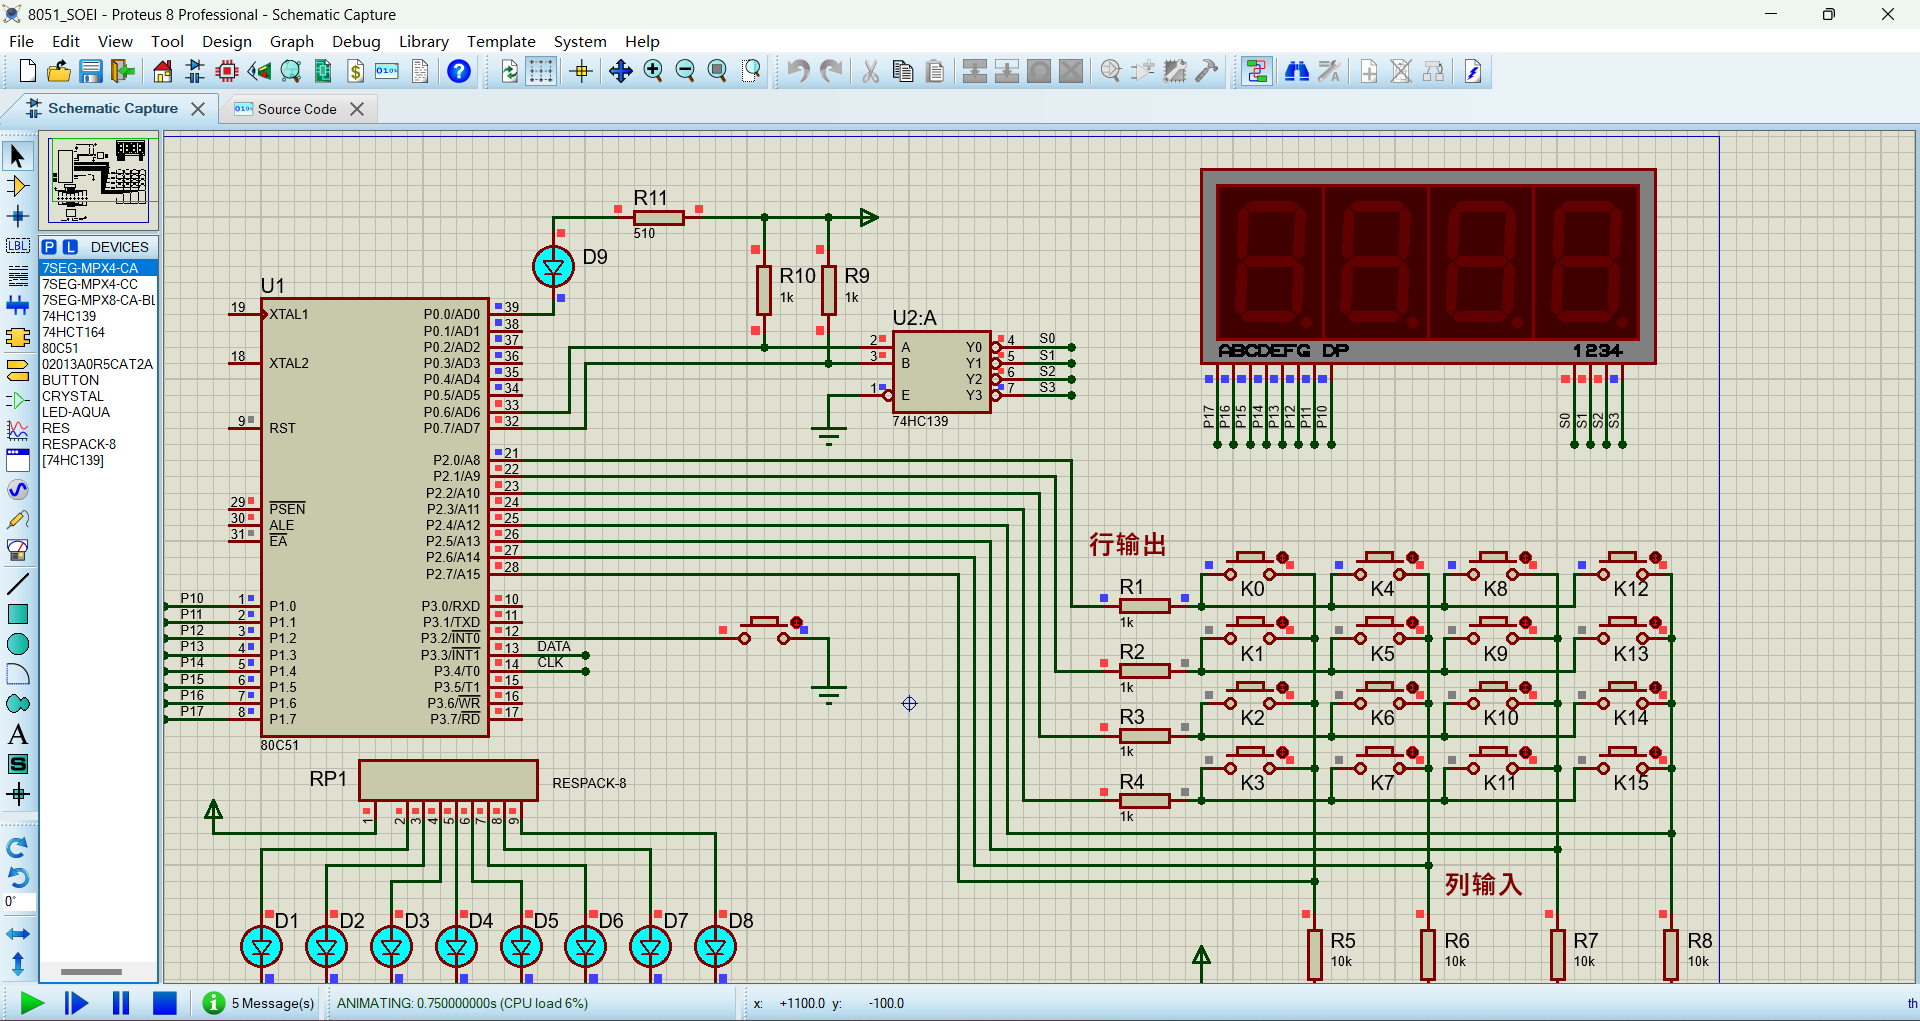
\includegraphics[width=0.78\textwidth]{figures/figure1.png}
    \caption{初始化与随机容量测试结果}
\end{figure}

\textbf{（2）分类按键开盖功能测试}

操作：以 P2.7 为例，将其拉低模拟“塑料纸张”投递按键。\\
预期：P1.0 拉低开盖，进入 8s 开盖窗口；若该桶未满则容量减 1。\\
结果：与预期一致。

\begin{figure}[H]
    \centering
    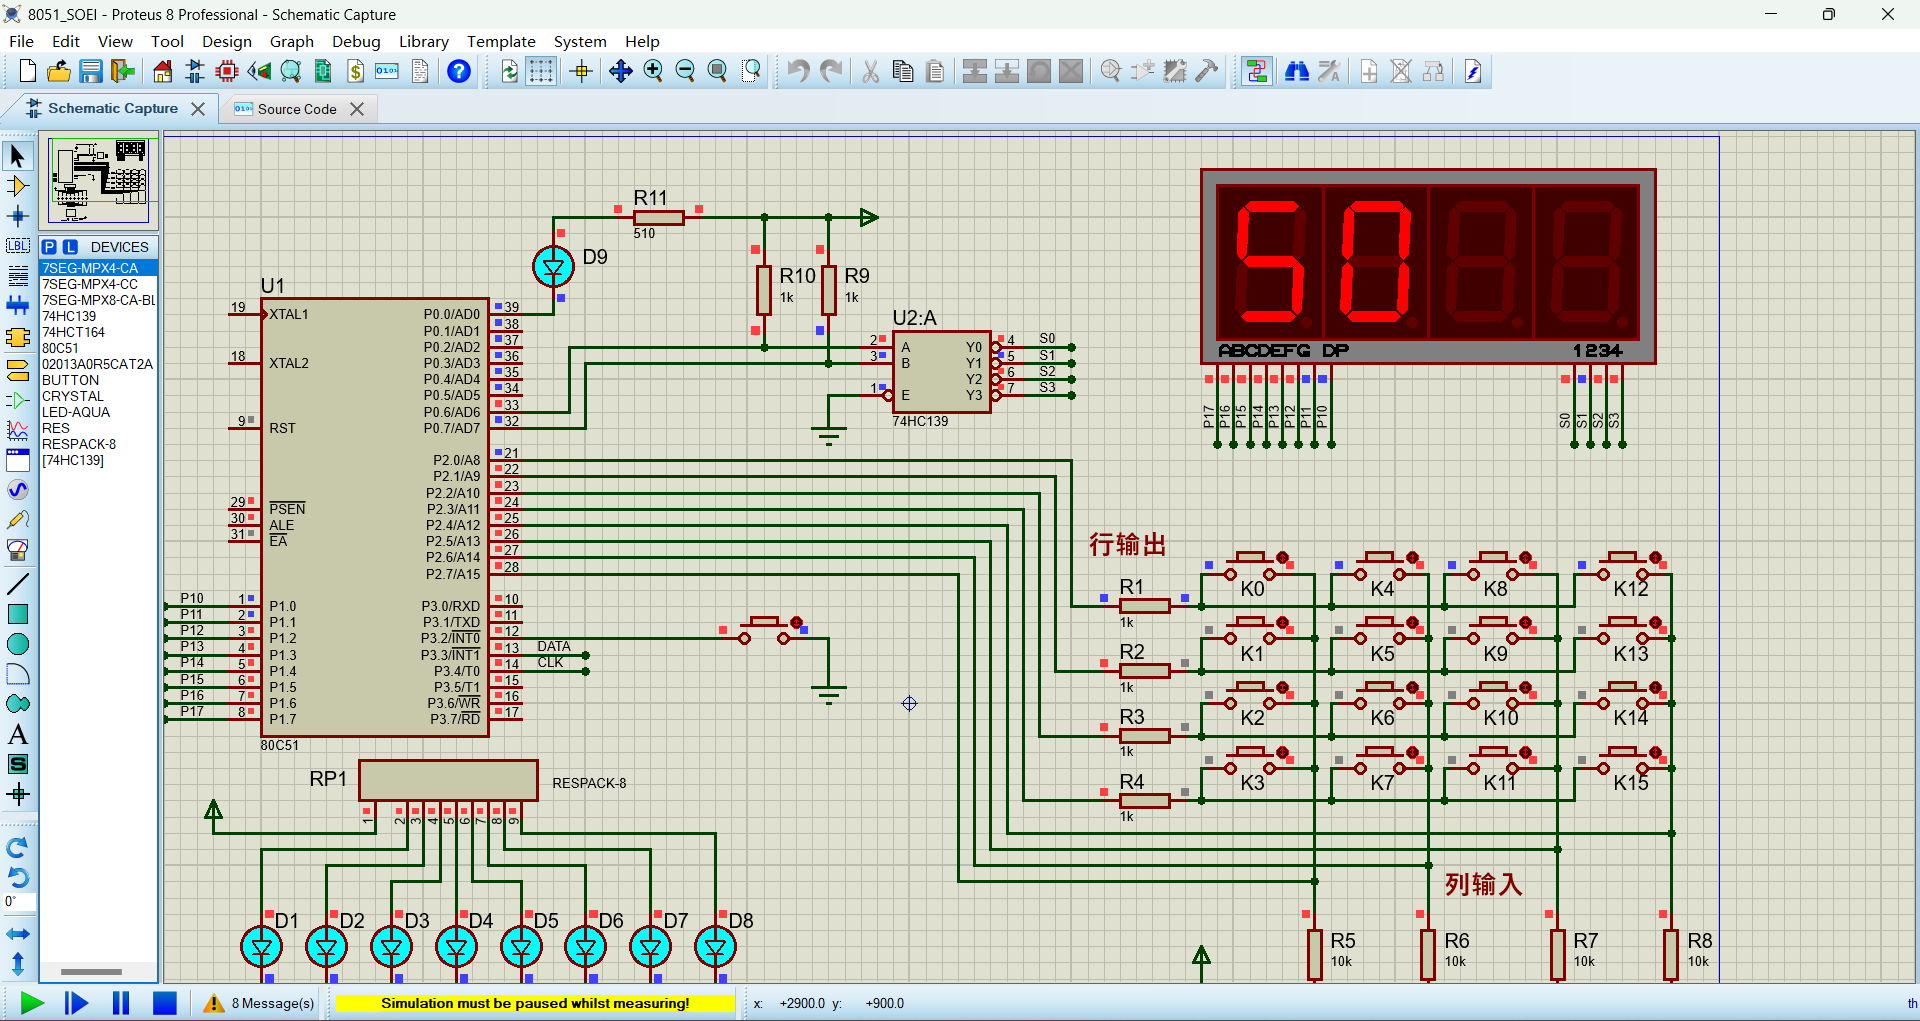
\includegraphics[width=0.78\textwidth]{figures/figure3.png}
    \caption{分类按键开盖测试结果}
\end{figure}

\textbf{（3）8秒自动关盖与P0进度条测试}

操作：触发任一垃圾桶开盖后，持续观察 Timer0 中断过程。\\
预期：每 1 秒 SEC\_LEFT 减 1，同时 P0 由 FFH 逐步右移至 00H；8 秒到期后自动调用 FORCE\_CLOSE，P1 对应位恢复高电平。\\
结果：与预期一致。

\begin{figure}[H]
    \centering
    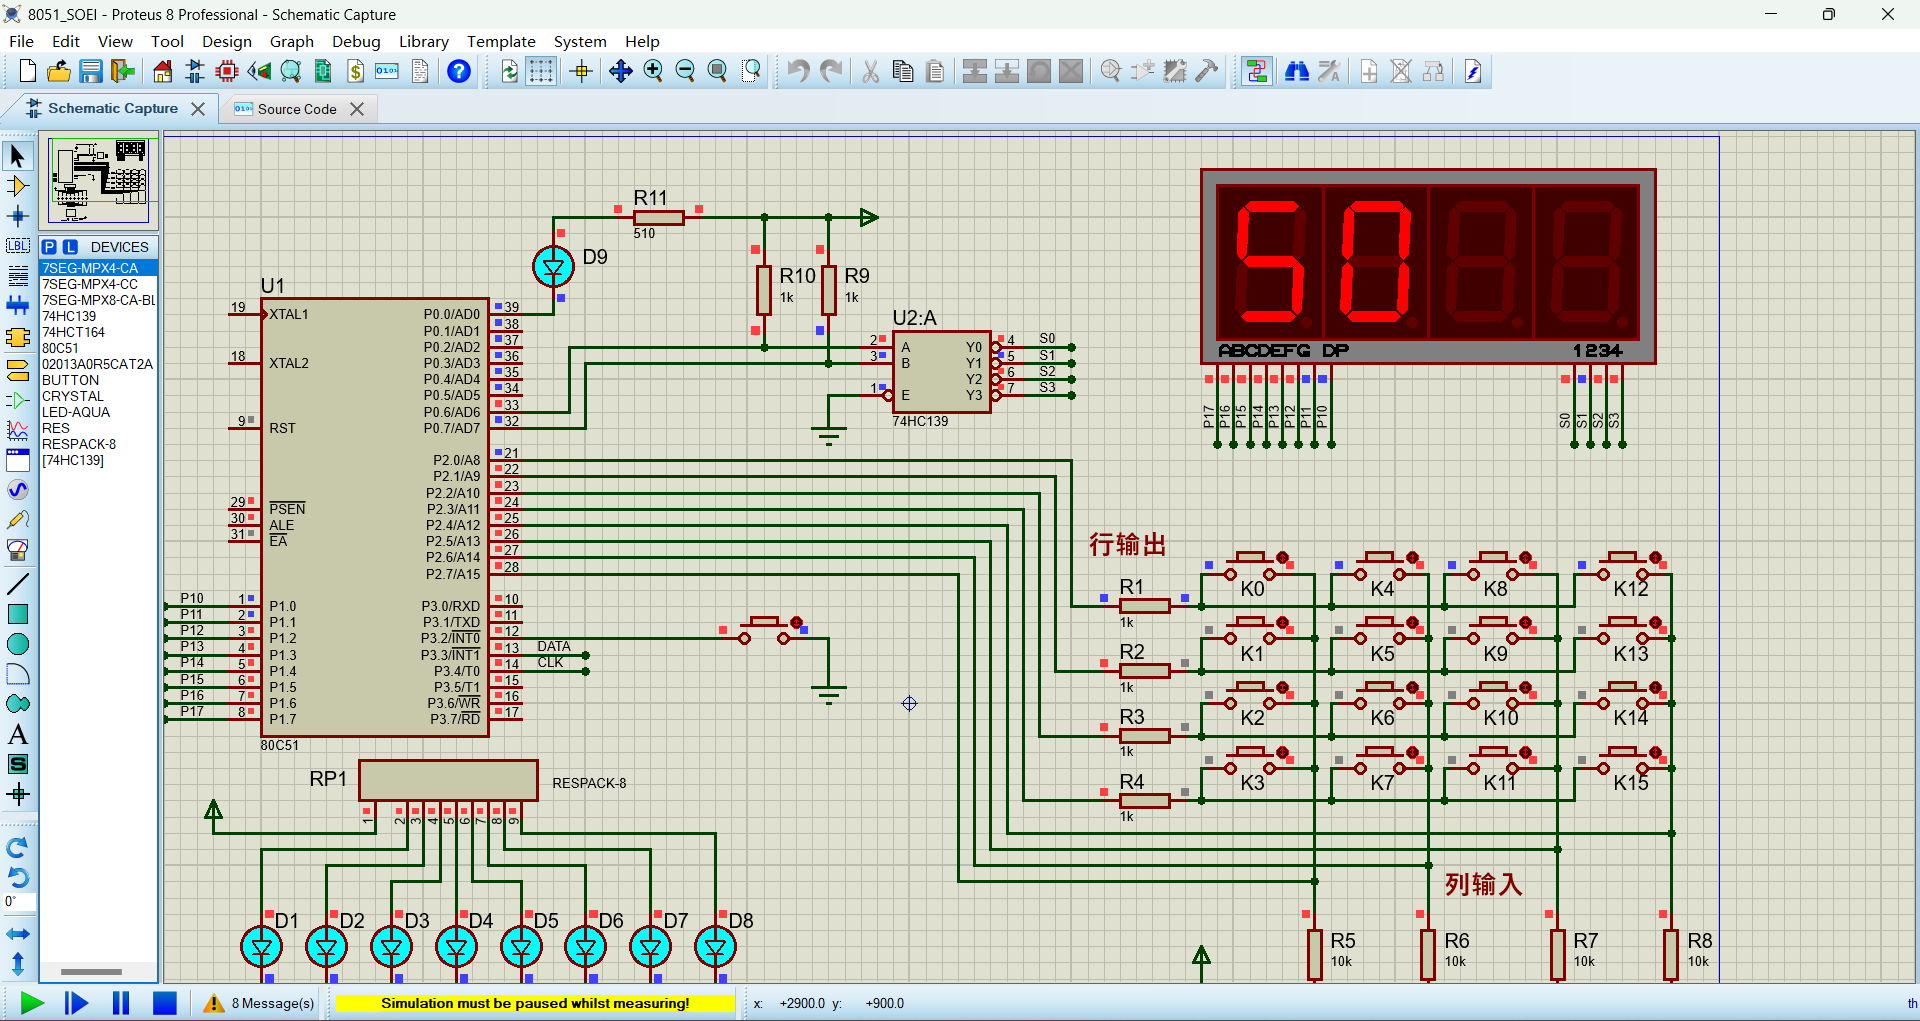
\includegraphics[width=0.78\textwidth]{figures/figure3.png}
    \caption{自动关盖与进度条测试结果}
\end{figure}

\textbf{（4）满载封桶与指示灯测试}

操作：连续投递使某一桶容量减至 0，并再次触发该桶按键。\\
预期：对应满载标志位置 1，后续按键不再开盖；满载指示口（P3.0/P3.1/P3.4/P3.5）对应位置高电平。\\
结果：与预期一致。

\begin{figure}[H]
    \centering
    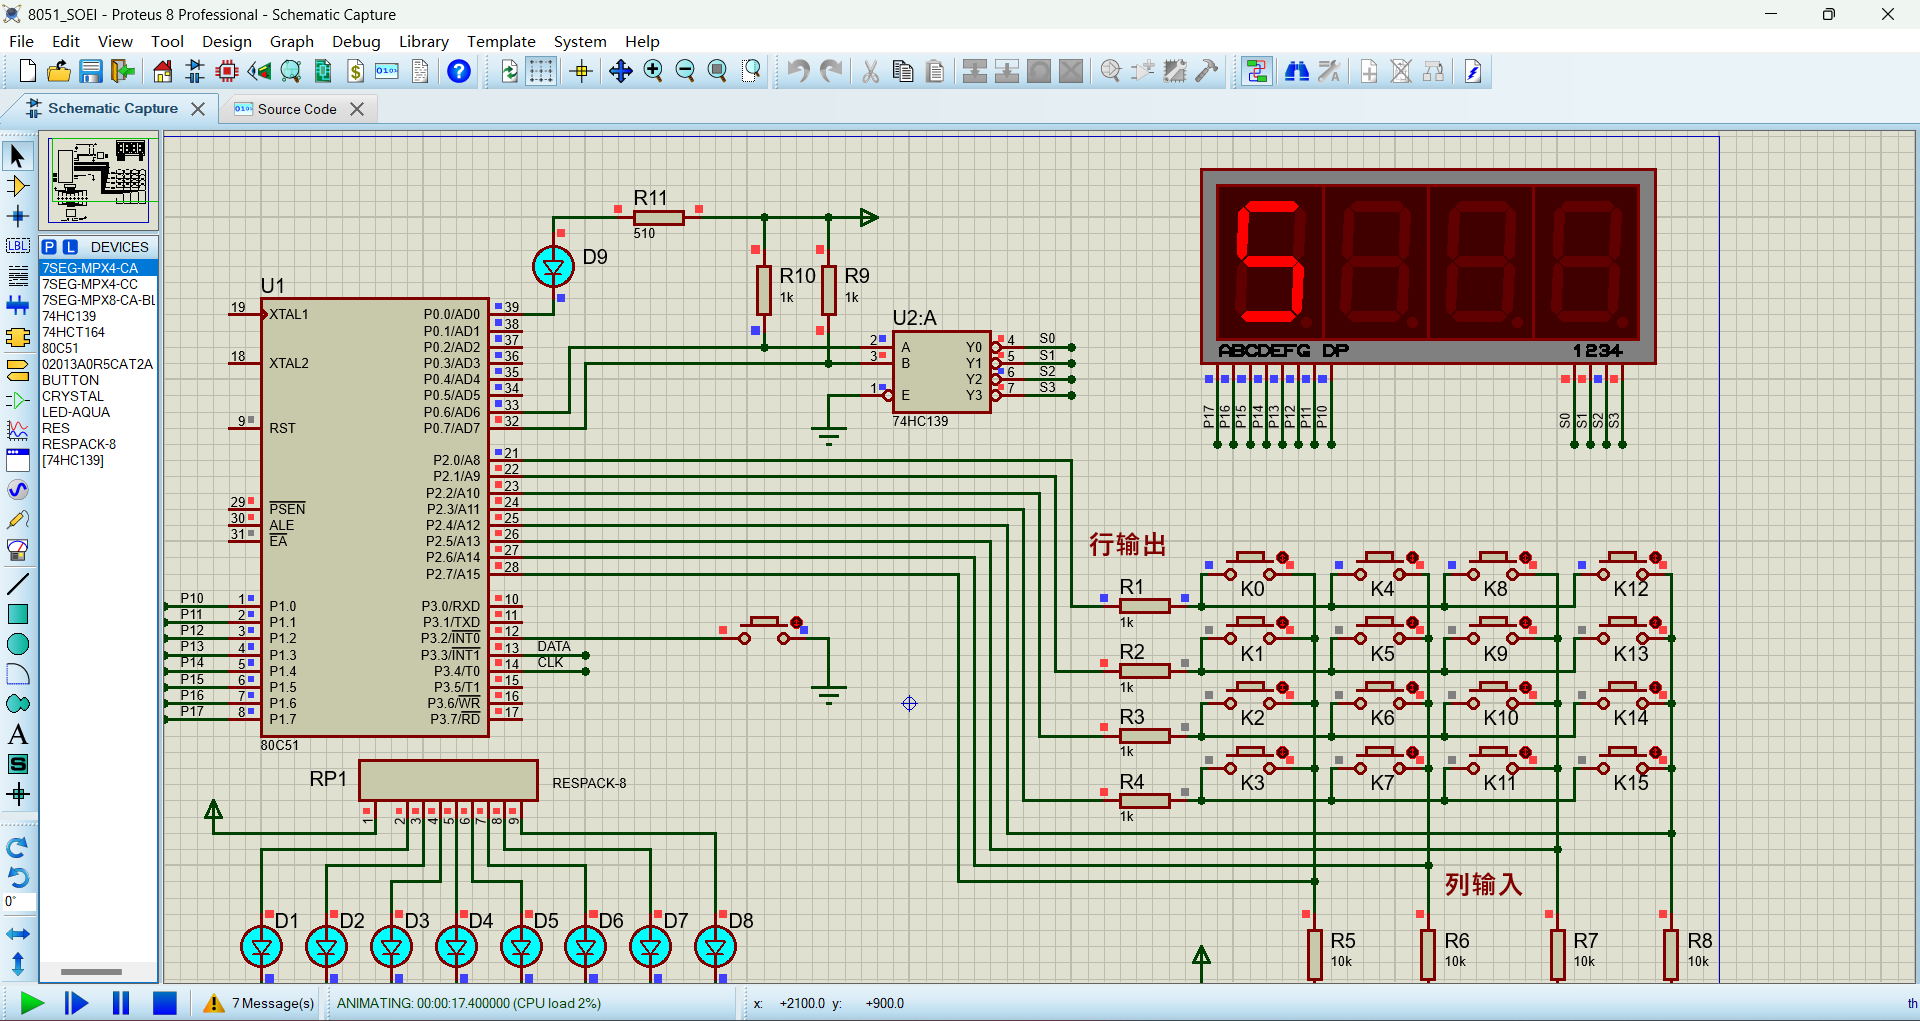
\includegraphics[width=0.78\textwidth]{figures/figure2.png}
    \caption{满载封桶测试结果}
\end{figure}

\textbf{（5）清理键复位测试}

操作：按下 P2.3 清理键。\\
预期：R0$\sim$R3 全部恢复为 9，FULL\_FLAGS 清零，满载指示熄灭。\\
结果：与预期一致。

\begin{figure}[H]
    \centering
    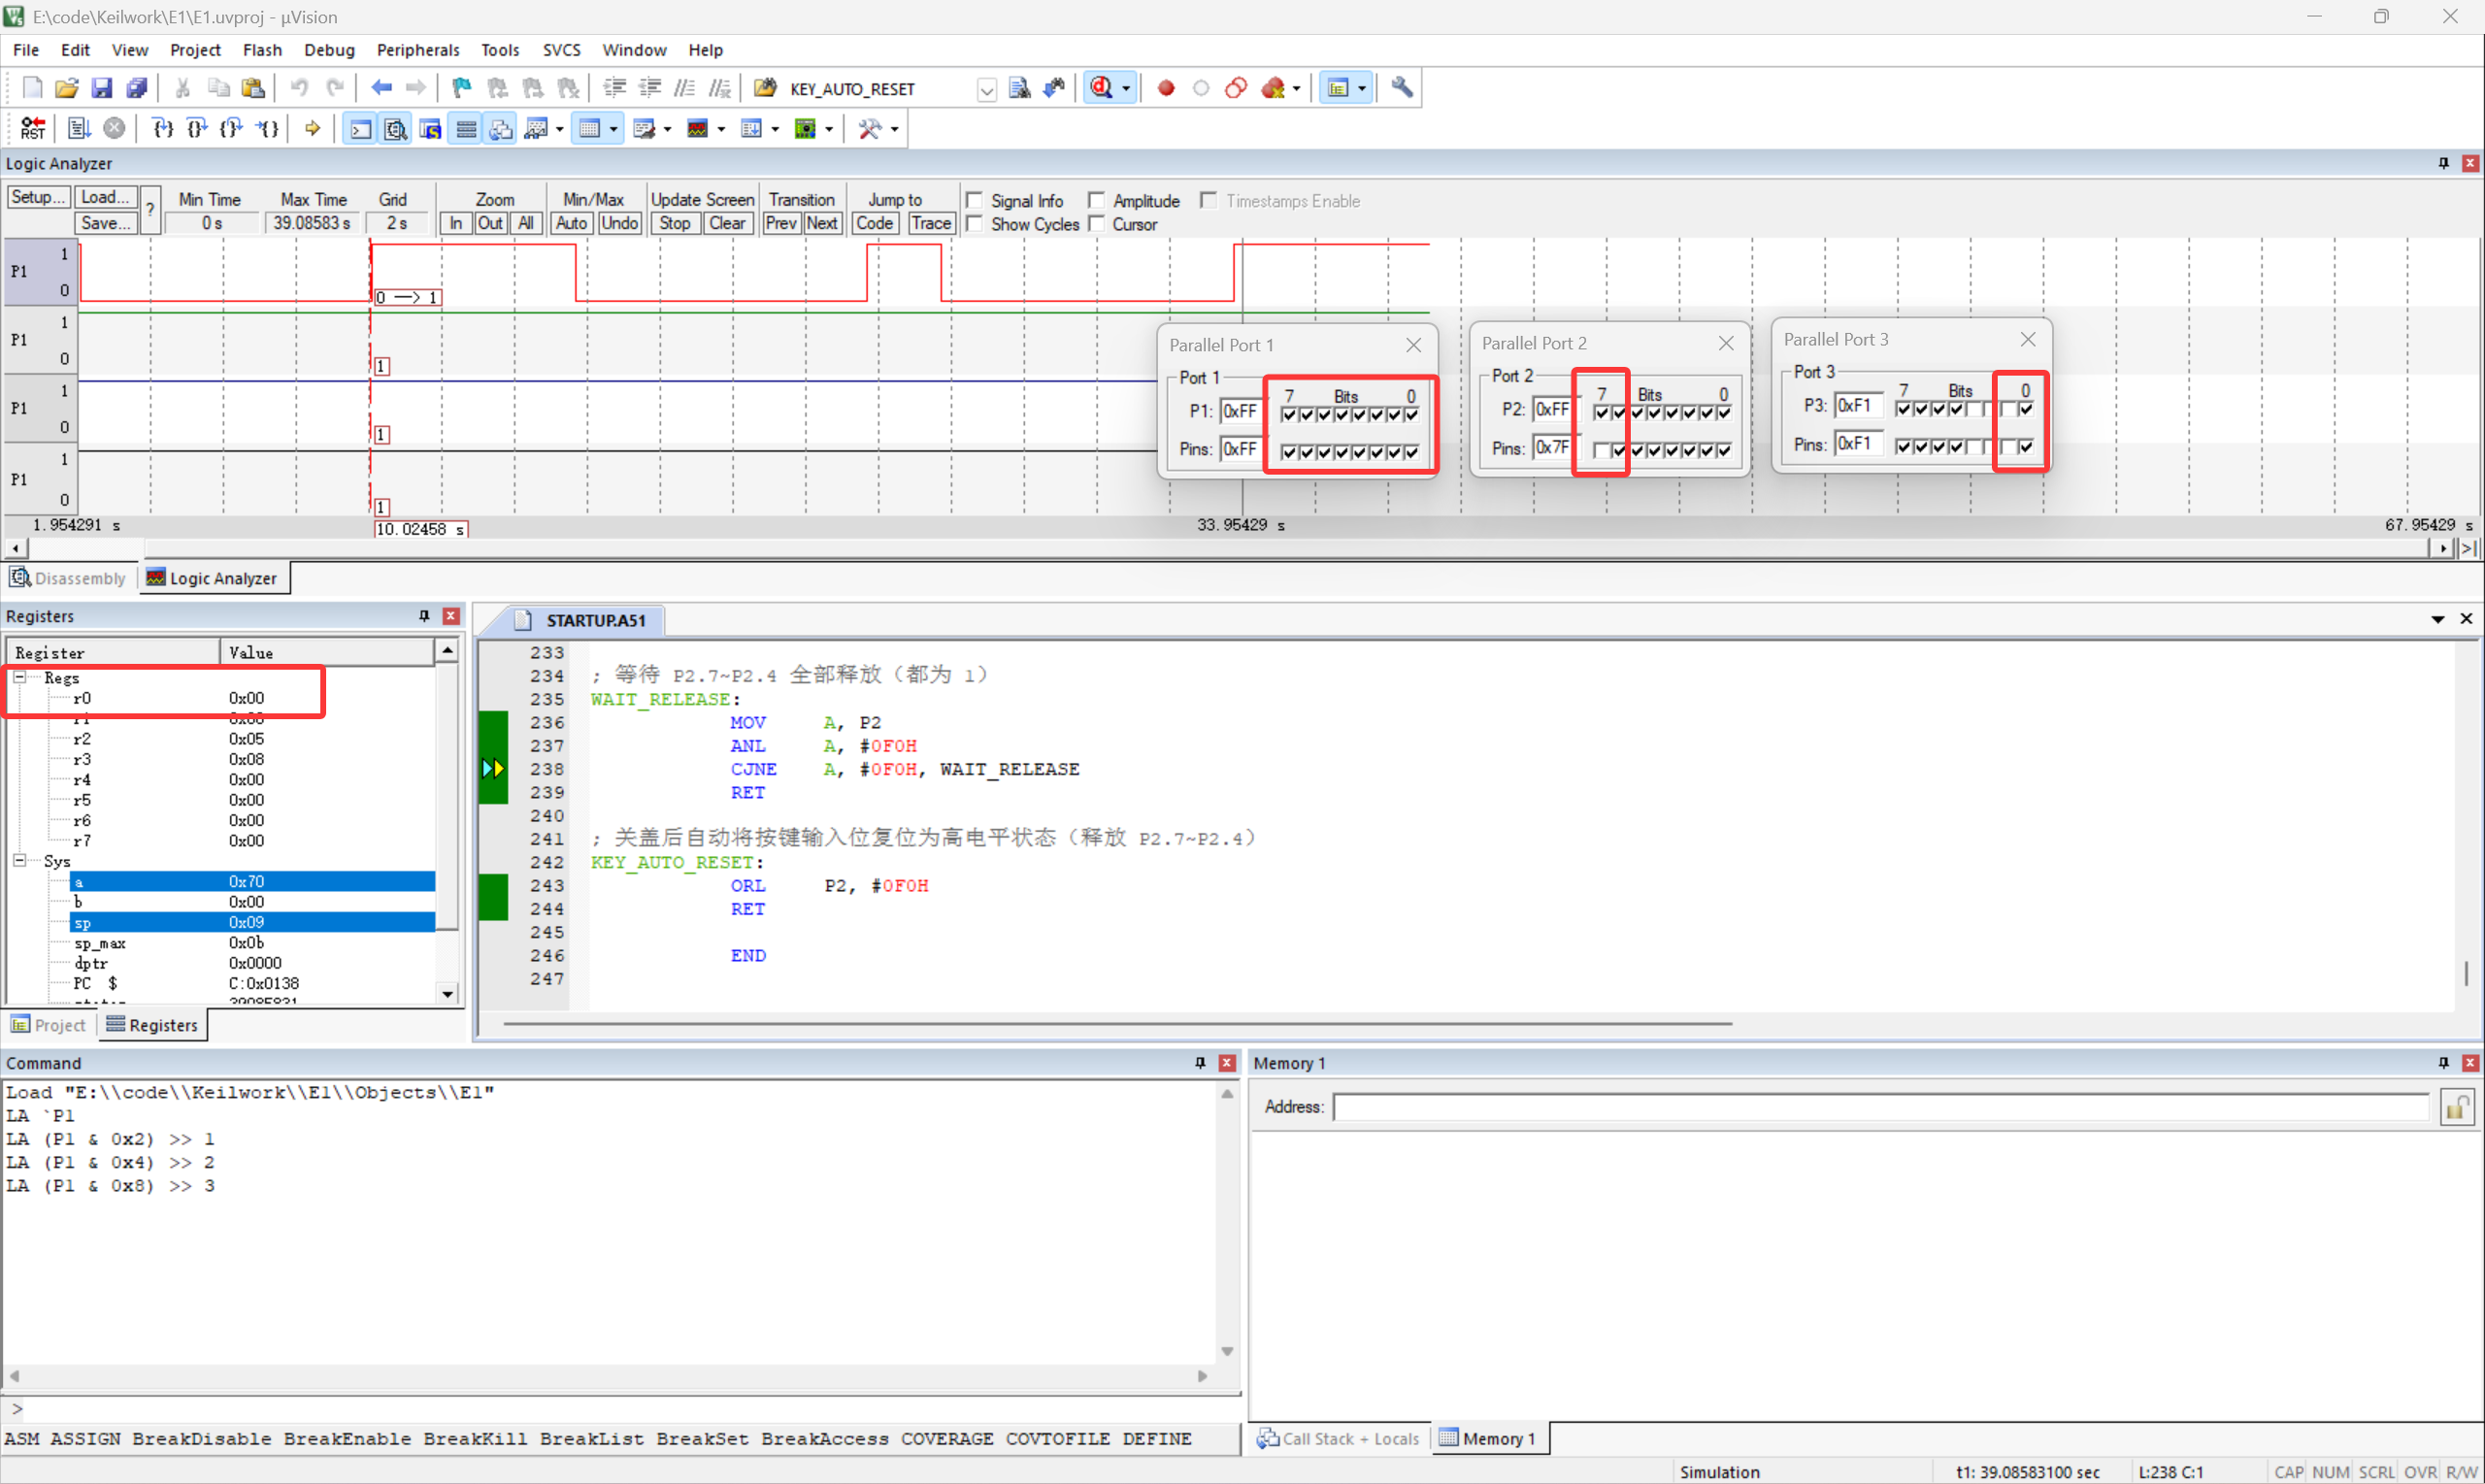
\includegraphics[width=0.78\textwidth]{figures/figure5.png}
    \caption{清理复位测试结果}
\end{figure}

\textbf{（6）INT0提前关盖中断测试}

操作：开盖窗口内触发 P3.2（INT0）下降沿中断。\\
预期：进入 EXT0\_ISR，立即调用 FORCE\_CLOSE，停止 T0 计时并提前关闭当前桶盖，OPENING 清零。\\
结果：与预期一致。

\begin{figure}[H]
    \centering
    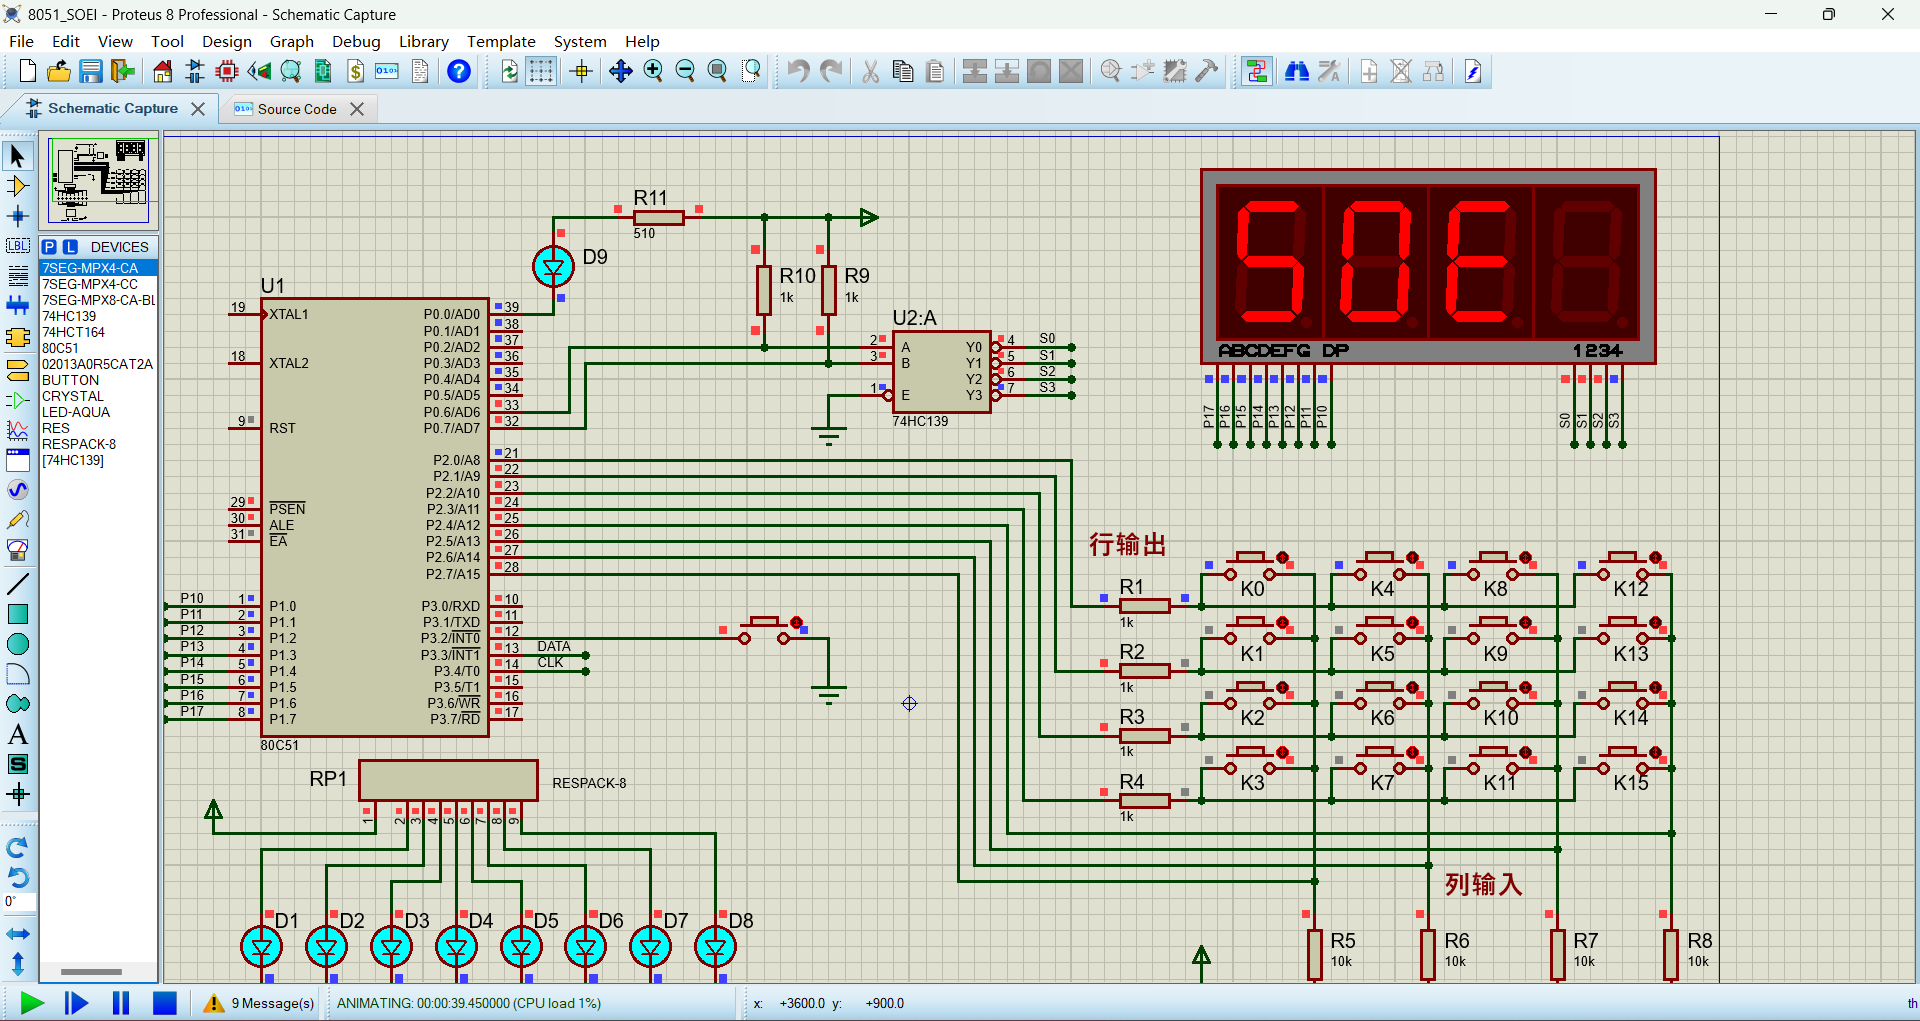
\includegraphics[width=0.78\textwidth]{figures/figure4.png}
    \caption{提前关盖中断测试结果}
\end{figure}

综上，程序已完成任务书要求的全部核心功能，并实现了容量管理、清理复位和中断提前关盖功能。




\section{实验问题分析与对策}

\begin{enumerate}
    \item \textbf{定时器1ms节拍精度问题}：
    \begin{itemize}
        \item \textbf{问题}：实验要求通过定时器中断实现8s开盖窗口，但在仿真的配置中误将晶振频率设置为24MHz，导致关盖时间只有4s，不符合设计要求。
        \item \textbf{对策}：将晶振频率调整为12MHz，确保代码逻辑与硬件外设保持一致，从而达到实验需求。
    \end{itemize}
    
    \item \textbf{提前关盖中断与端口复用冲突问题}：
    \begin{itemize}
        \item \textbf{问题}：提前关盖采用INT0时必须占用P3.2，而原方案将P3.0$\sim$P3.3全部用于满载指示，导致引脚功能冲突。
        \item \textbf{对策}：将P3.2专用于INT0下降沿触发，满载指示调整为P3.0、P3.1、P3.4、P3.5。并在UPDATE\_FULL\_LED中完成位映射，确保中断输入与指示输出互不干扰。
    \end{itemize}

    \item \textbf{按键连发与释放判定问题}：
    \begin{itemize}
        \item \textbf{问题}：低电平按键在未释放时会被主循环重复识别，造成一次按压触发多次投递分支。
        \item \textbf{对策}：所有投递分支和清理分支结束前统一调用WAIT\_RELEASE，等待相关按键恢复高电平后再返回主循环，抑制连发，提高交互稳定性。
    \end{itemize}

\end{enumerate}

\vspace{2cm}
\noindent
本人承诺:本报告内容真实，无伪造数据，无抄袭他人成果。本人完全了解学校相关规定，如若违反，愿意承担其后果。

\vspace{1cm}
\noindent
签字：\hspace{3cm} 陈恪瑾 \hspace{3cm} 2026年4月26日

\end{document}
